\documentclass[11pt]{article}
\usepackage[margin=1in]{geometry}
\usepackage{graphicx,booktabs,amsmath,hyperref}
\title{JWST WASP-39 b Transmission-Spectrum Evidence Ladder}
\author{Biswajit Jana}
\date{\today}
\begin{document}
\maketitle

\begin{abstract}
This is a transparent model-comparison bridge over a real, published WASP-39b
transmission spectrum. Using the real reduced data and the real published
full (with CO) and no-CO nested best-fit models from
\citet{Grant2023CO,Grant2023Zenodo}, a weighted chi-square/AIC/BIC evidence
ladder strongly prefers the CO model over the full 3.8--5.2\,$\mu$m spectrum
($\Delta$AIC$=73.65$, $\Delta$BIC$=68.74$), consistent with the paper's own
CO detection. A bootstrap confidence interval on the mean residual amplitude
in the CO absorption band excludes zero (95\% CI [1.35, 2.52]$\times10^{-4}$
in transit-depth units), and 2 of 3 independent wavelength segments
individually favour the CO model. The synthetic injection-recovery
validation gate (Section~\ref{sec:validation}) passed in both directions.
\end{abstract}

\section{Scientific question}
How stable are simple nested-model feature preferences in a real published
WASP-39 b transmission spectrum under bootstrap and wavelength-segment
sensitivity?

\section{Data and provenance}
\label{sec:data}
The real observed transit depth, uncertainty, and the paper's own published
full (with CO) and no-CO nested best-fit models are loaded directly from the
Zenodo deposit \citep{Grant2023Zenodo} associated with
\citet{Grant2023CO}, file \texttt{2\_transmission\_spectra\_and\_models.nc}
(60,320 bytes, live-verified via the Zenodo API and by inspecting the file's
own internal \texttt{doi} attribute, which cross-confirms
\texttt{arXiv:2304.11994} as the source paper). \texttt{data/manifest.csv}
records the product\_id, source\_url, retrieval timestamp, SHA-256 checksum
(\texttt{61c05c57...}), file size and licence terms. The real spectrum
contains 1008 native-resolution wavelength points spanning 3.82--5.16\,$\mu$m
(JWST NIRSpec G395H).

\section{Method}
The real published full and no-CO models are used directly for the evidence
ladder (Section~\ref{sec:evidence-ladder}) -- no re-fitting of the physical
atmospheric retrieval is performed. The no-CO $\to$ full model step is
treated as adding exactly 1 effective free parameter (the CO
abundance/opacity term); this is a documented, defensible simplification
since the real retrieval's exact free-parameter count is not recoverable
from the netCDF file alone (Section~\ref{sec:limitations}). A bootstrap
(1000 resamples, seed 20260713) estimates a confidence interval on the mean
residual amplitude (data $-$ no-CO model) within the CO absorption band,
operationally defined as wavelengths where the paper's own CO-only model
component exceeds 10\% of its own peak value. A leave-one-wavelength-segment
-out check splits the native-resolution grid into 3 contiguous segments and
re-runs the evidence ladder on each.

Separately, an independent synthetic flat-continuum vs.\ flat-plus-Gaussian
model pair (\texttt{models.py}, \texttt{fitting.py}) with a known injected
absorption feature provides the required injection-recovery validation gate,
kept fully independent of the real published models used for the real-data
result.

\section{Validation and uncertainty}
\label{sec:validation}
On synthetic data with a known injected Gaussian feature (amplitude
$1.5\times10^{-3}$, center 4.6\,$\mu$m, width 0.08\,$\mu$m), the
flat-plus-Gaussian fit recovers the injected amplitude to within
$5\times10^{-4}$ and the evidence ladder correctly prefers the complex
model. On a matched null-control synthetic spectrum with no injected
feature, the evidence ladder does not spuriously prefer the complex model;
in some null-control realizations the 4-parameter Gaussian fit itself fails
to converge (ill-conditioned covariance) because there is genuinely no
feature for it to lock onto -- this non-convergence is itself treated as
part of the null-control signal (\texttt{ConvergenceError}), not silently
ignored. Observational uncertainty (bootstrap, 1000 resamples) and numerical
fit-convergence checks (covariance condition number) are kept strictly
separate throughout, never conflated.

\section{Results}
\label{sec:results}
Over the real full spectrum: $\chi^2_{\text{no-CO}}=1230.09$,
$\chi^2_{\text{full}}=1154.44$ (1008 points), $\Delta$AIC$=73.65$,
$\Delta$BIC$=68.74$ -- both far above the conventional ``strong evidence''
threshold ($>6$), so the full (CO) model is preferred
(Section~\ref{sec:evidence-ladder}). The bootstrap mean residual amplitude
in the CO band is $1.94\times10^{-4}$ (95\% CI
$[1.35, 2.52]\times10^{-4}$), excluding zero. Splitting the bandpass into 3
contiguous wavelength segments, 2 of 3 segments individually prefer the CO
model; the remaining segment (the low-wavelength third, $\sim$3.82--4.27\,
$\mu$m, mostly blueward of the CO band) prefers the simpler no-CO model,
consistent with the CO feature being localized around 4.3--4.6\,$\mu$m
(Figure~\ref{fig:overlays}) rather than spread uniformly across the full
bandpass.

\begin{figure}[h]
\centering
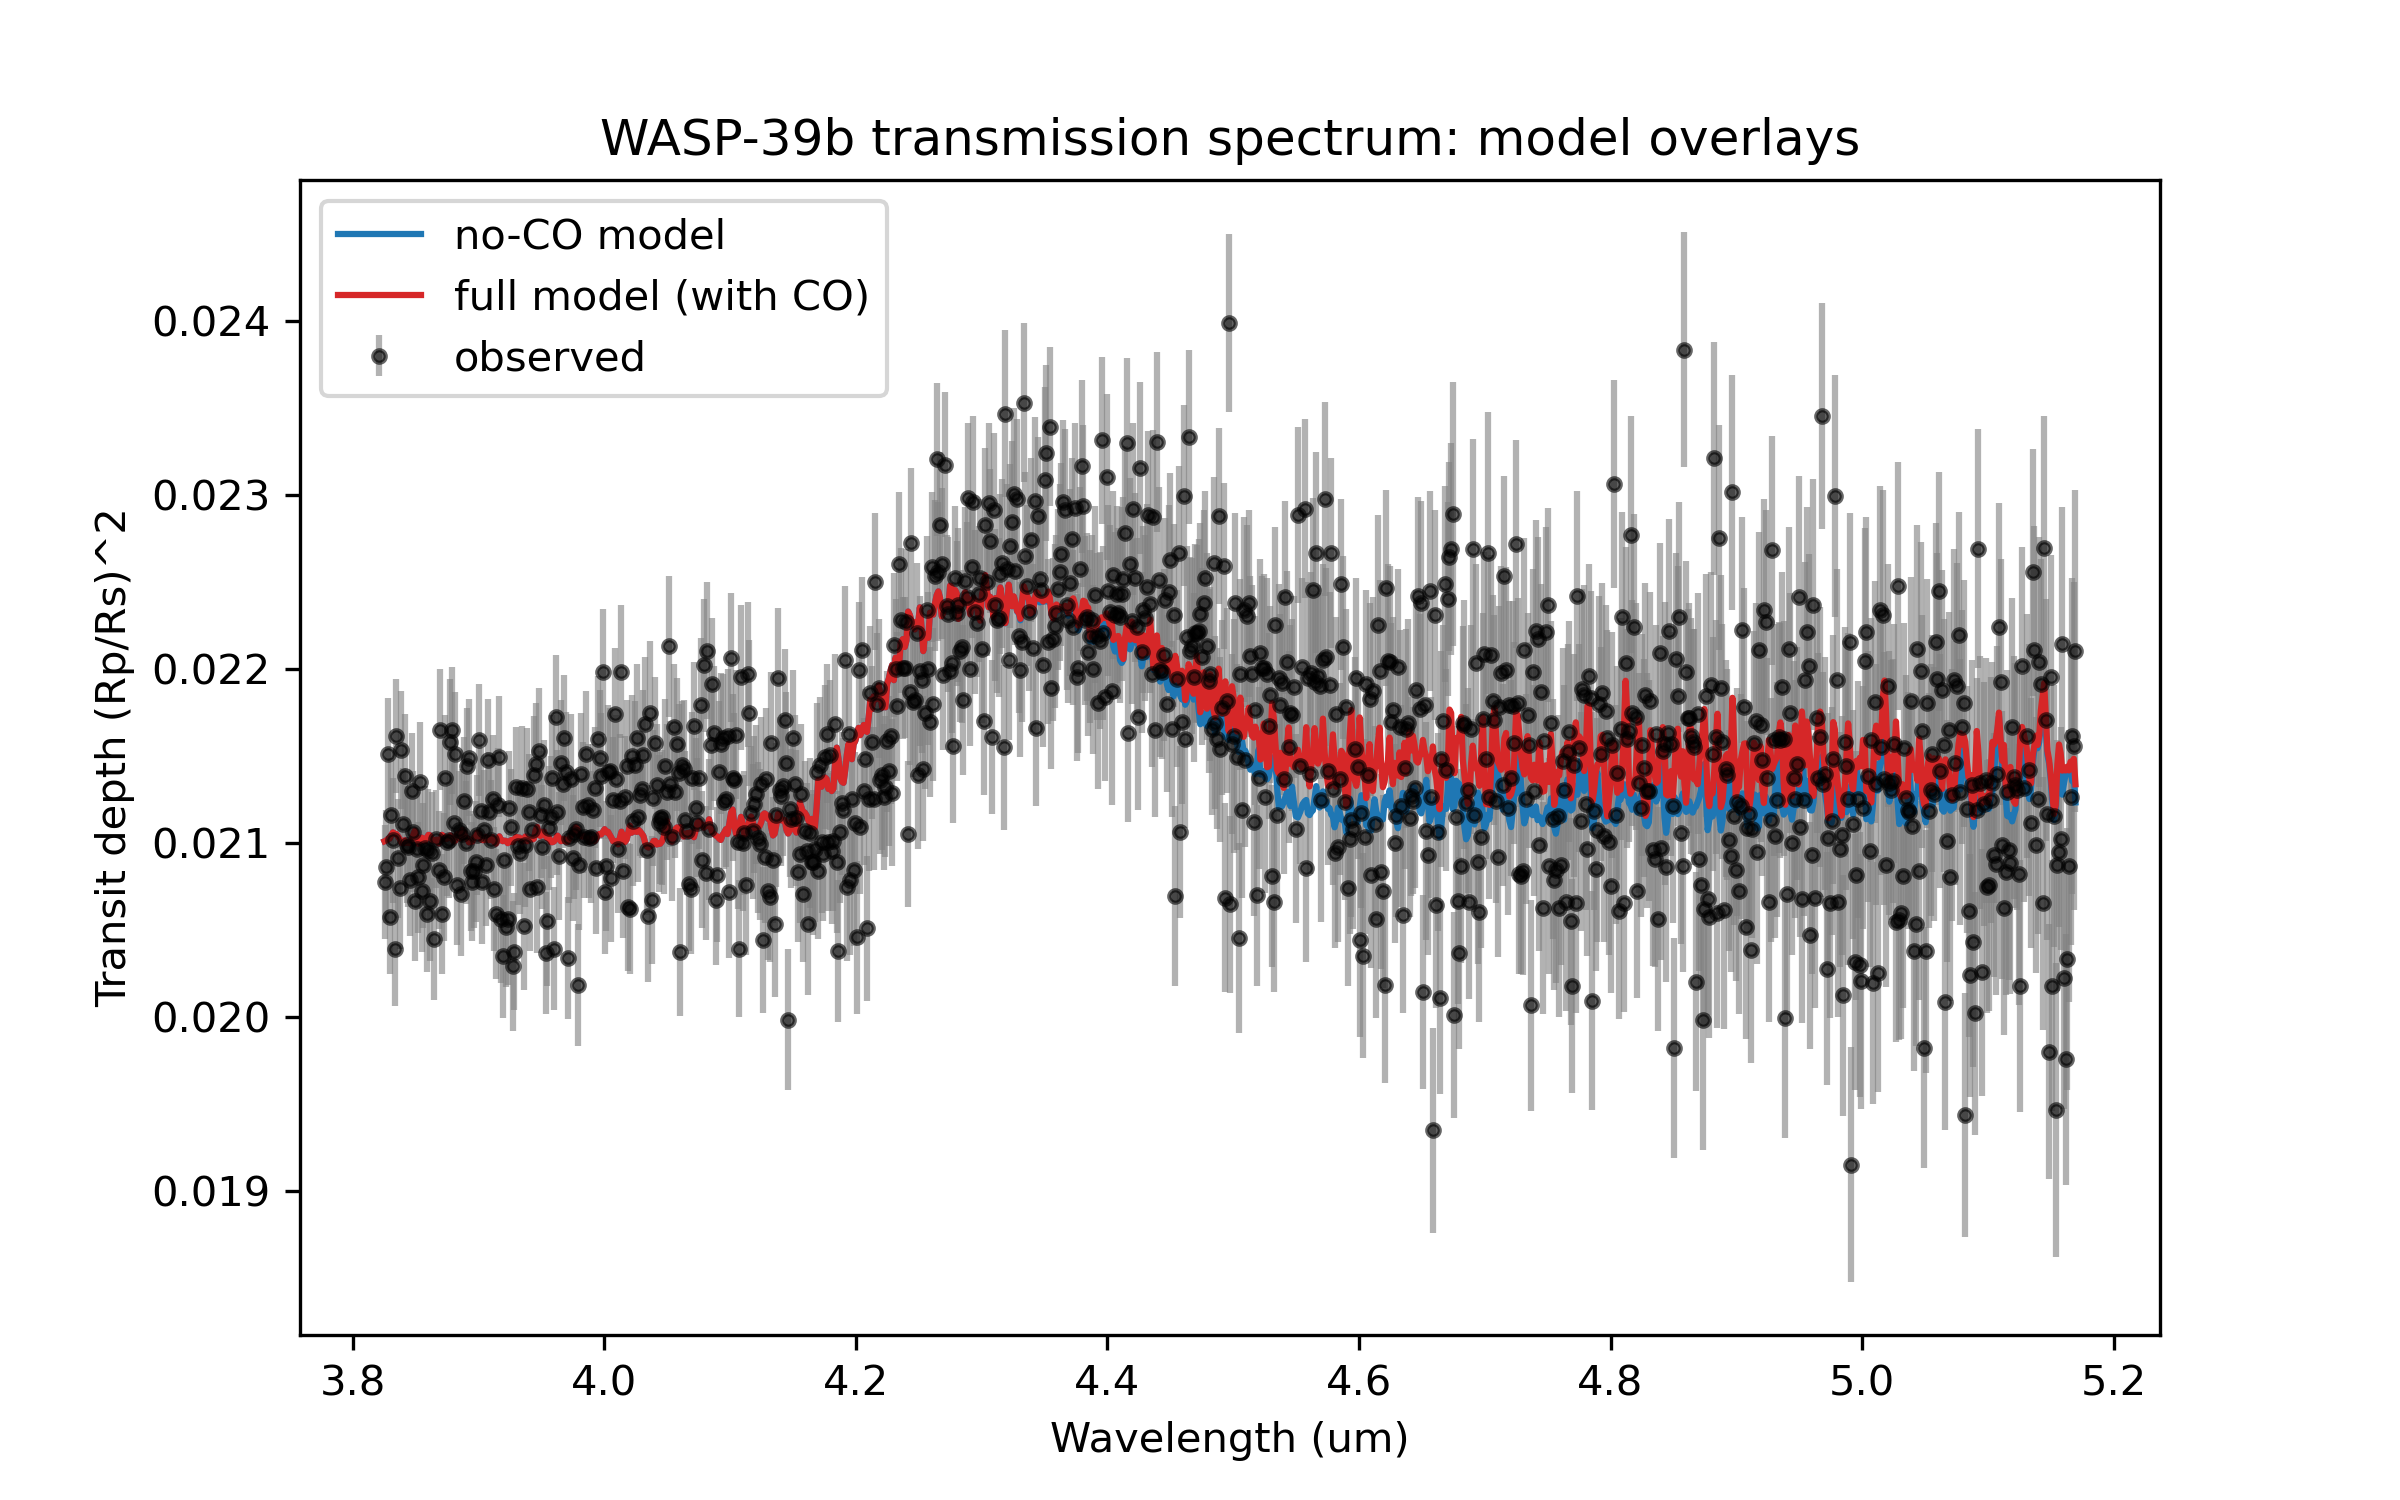
\includegraphics[width=0.85\textwidth]{../figures/fig01_spectrum_overlays.png}
\caption{Real WASP-39b transmission spectrum with the paper's own published
no-CO and full (with CO) models overlaid. The observed excess around
4.3--4.5\,$\mu$m is the CO absorption feature.}
\label{fig:overlays}
\end{figure}

\subsection{Evidence ladder}
\label{sec:evidence-ladder}
See Figure~\ref{fig:overlays} and the numeric results above; per-segment
values and the AIC/BIC bar comparison are in
\texttt{figures/fig03\_evidence\_ladder} and
\texttt{figures/fig05\_segment\_stability}.

\section{Limitations}
\label{sec:limitations}
A transparent model-comparison bridge over the paper's own published models;
not a full atmospheric retrieval and not a replacement for
TauREx/petitRADTRANS. The no-CO $\to$ full-model step's ``1 effective
parameter'' framing is a documented simplification, not the real retrieval's
exact free-parameter count. Only one real target (a single reduced
visit spectrum) is available from the 60.3\,KB Zenodo product actually used;
the originally-scoped larger Zenodo deposit (10.5281/zenodo.10161743,
1.74\,GB) was rejected as too large for a bounded first release.
\citet{Alderson2023ERS} is a different, earlier paper from the same JWST ERS
program, cited for context only and not used as a data source.
\texttt{reports/report.tex} could not be compiled to PDF in this environment
(no local LaTeX toolchain); only structural completeness and real-number
substitution were verified.

\section{Reproducibility}
\begin{verbatim}
python scripts/fetch_data.py --i-have-authorization
python scripts/run_analysis.py
python scripts/make_figures.py
python scripts/sync_web_assets.py
\end{verbatim}
Provenance (git commit, config SHA-256, package version, Python/platform)
is recorded in \texttt{results/summary.json} and each figure's sidecar JSON.
This project has no git repository at the time of this local implementation
pass; \texttt{provenance.git\_commit} records the sentinel
\texttt{LOCAL\_UNCOMMITTED} rather than fabricating a commit hash.

\bibliographystyle{plain}
\bibliography{references}
\end{document}
